\subsection{Gallery of Model Fits to Supra-threshold Experiments}
\begin{comment}
\begin{figure}
    \centering
    \begin{subfigure}[t]
        \centering
        \includegraphics[width=0.5\linewidth]{example-image-a.pdf} 
        \caption{Generic} \label{fig:timing1}
    \end{subfigure}
    \hfill
    \begin{subfigure}[t]
        \centering
        \includegraphics[width=0.5\linewidth]{example-image-b.pdf} 
        \caption{Competitors} \label{fig:timing2}
    \end{subfigure}

    \vspace{1cm}
    \begin{subfigure}[t]
        \centering
        \includegraphics[width=0.5\linewidth]{example-image-c.pdf} 
        \caption{Price regulation} \label{fig:timing3}
    \end{subfigure}
    \hfill
    %\begin{subfigure}[t]%{0.45\textwidth}
    %    % just an empty subfigure to shift C below A
    %\end{subfigure}
    \caption{Some general caption of all the figures. In (\subref{fig:timing1}) you can see a  green square....}
\end{figure}
\end{comment}

% TODO make multi panel.

\begin{figure}
    \centering
    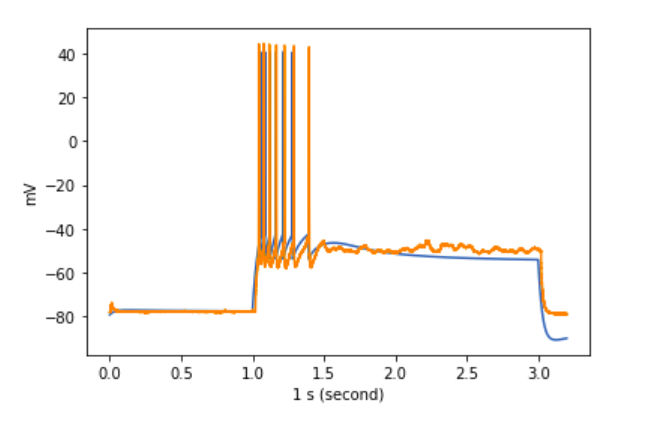
\includegraphics[scale=0.75]{figures/adexp_fit_allen_spec_id_476053392.png}
    \caption{An adaptive Exponential Model was fitted to both the spike time, and spike shape data in a sweep from Allen specimin id: 476053392} \label{fig:specimen_476053392}
\end{figure}

\begin{figure}
    \centering
    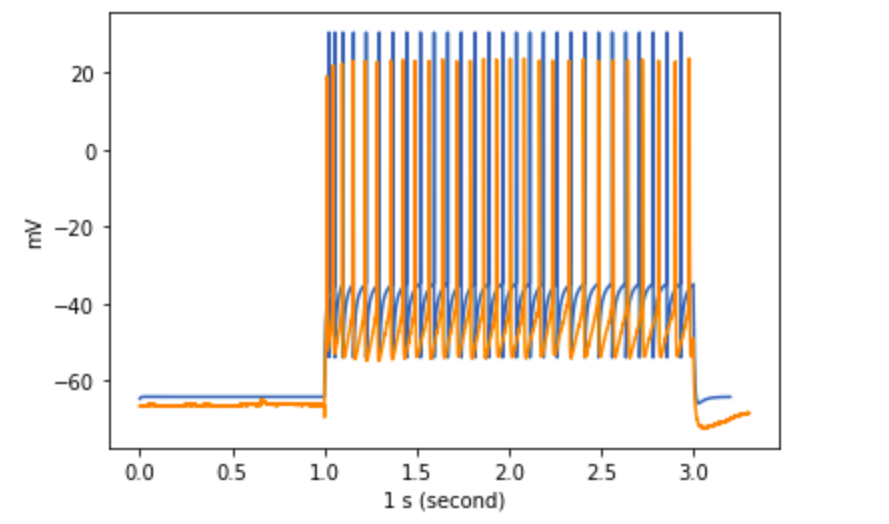
\includegraphics[scale=0.75]{figures/28spikesB95}
    \caption{An adaptive Exponential Model was fitted to both the spike time, and spike shape data in a sweep from Allen specimin id: 476053392} \label{fig:specimen_476053392}
\end{figure}

%Similar to Druckmann Suprathreshold depolarizing step currents \cite{druckmann2008evaluating}.
\begin{figure}
    \centering
    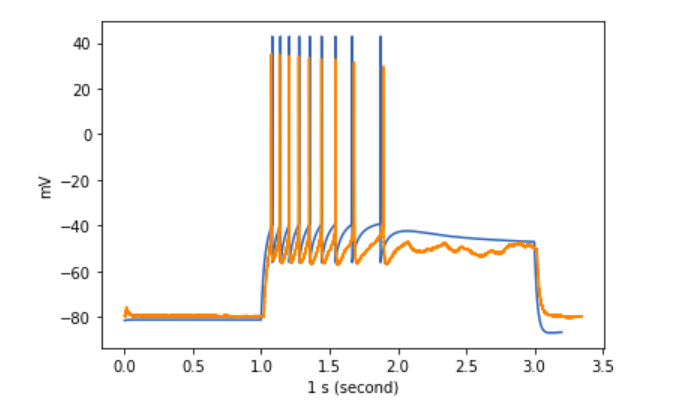
\includegraphics[scale=0.75]{figures/adexp_fit_allen_specid_325479788.png}
    \caption{ An adaptive Exponential Model was fitted to both the spike time, and spike shape data in a sweep from Allen specimin id: 325479788}
    \label{fig:specimen_325479788}
\end{figure}


% Interesting direct qoute from Druckmann:
%"In experiments, intrinsic noise gives rise to a large variability (e.g., in firing pattern) in the voltage responses to repetitions of the exact same input. Thus, the common approach of fitting models by attempting to perfectly replicate, point by point, a single chosen trace out of the spectrum of variable responses does not seem to do justice to the data."

%In experiments, however, when the exactly same stimulus is repeated several times, the voltage traces elicited differ among themselves to a significant degree (Mainen and Sejnowski, 1995; Nowak et al., 1997).

A joint collection of current injections and recordings known as sweeps were taken from a rat somato-sensory hind limb neuron.
\ref{fig:B95Adexp} is a challenging waveform to fit, as adaption does not predict the final ISI, which is smaller than the penultimate one. 

Although it is not obvious there is significant variation in ISIs (although the range of that variation may be concentrated within a small margin). As noted in the literature \cite{druckmann2007novel} it is probably mis-founded to over fit models to exact spike times because neurons themselves experience noisy intrinsic currents and they are likely to illicit different spike trains, given identical presentation of stimulus. In hind-sight I propose, to optimize on FI-slope and spike rate, while comprimizing on exact spike time agreement.

\begin{figure}
    \centering
    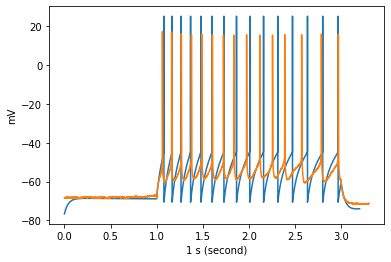
\includegraphics[scale=0.75]{figures/bbp_multispiking_fit.png}
    \caption{An adaptive Exponential Model was fitted to both the spike time, and spike shape data in a sweep from animal B95 
    %\url{http://microcircuits.epfl.ch/#/animal/8ecde7d1-b2d2-11e4-b949-6003088da632}
    Blue Brain Project. The base voltage. The base voltage, and Resting Membrane Potential, and spike numbers are matched, spike times are not perfectly aligned, spike height, and trough depth are not perfectly matched}
    \label{fig:B95Adexp}
\end{figure}

\begin{figure}
    \centering
    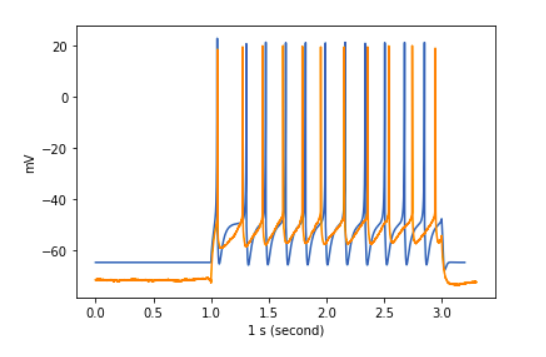
\includegraphics{figures/IZHI_B95.png}
    \caption{An Izhikevich model was fitted to both the spike time, and spike shape data in a sweep from Blue Brain Project. The Spike amplitude, and spike numbers are matched, spike times are not perfectly aligned. Although this optimisation solution obviously resulted in some misaligned spike times, bare in mind, that the some of the best optimized models only predict $86\%$ of spike times at best, and that is when they are supplied with some highly specific excitatory and inhibitory currents}
    \label{fig:B95_IZHI}
\end{figure}

In figures \ref{fig:B95Adexp}, you can see that although several aspects of the waveform are fitted, exact spike times are not always fitted \ref{fig:B95_IZHI}

The result that the adaptive exponential model is better able to fit spike times than the Izhikevich model is consistent with the literature \cite{rossant2011fitting}. the figure below shows results from the INCF modelling competition the adaptive exponential model and families of models related to it such as the MAT model (made to order Multiscale Adaptive Time window) model, are significantly better able to fit to spike times than the Izhikevich model.



\begin{figure}
    \centering
    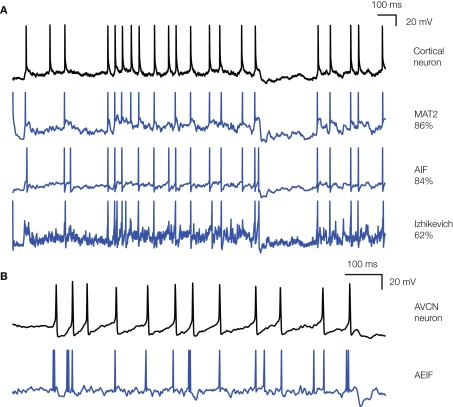
\includegraphics[scale=5.0]{figures/IZHIkevich_fit_60Adexp_80.jpg}
    \caption[The spectrum of model fits]{This figure from the publication: \cite{rossant2011fitting} shows how the majority of models that fit spike time, do not also fit spike shape. Spike shape and AP timing constitute a persistent conflicted priority with regards to model fitting. Included in this figure are fits from reduced models used in this work. Including the Izhikevich model, and the AIF model (herein referred to as AdEx). In this  context the MAT2 model correctly predicts $86$ of spike times, but you can see that the spike threshold is much higher in the model compared to the experiment. The Izhikevich model only predicts $62\%$ of spike times (this is also consistent with my results), and it displays much more below threshold activity than the data and the other models.} 
    \label{fig:my_label}
\end{figure}